\section{Constructing topics using human judgments}
\label{sec:tasks}
One can replace the collapsed Gibbs sampling equation given as
\myeq{eq:sampling} with any other sampling equation, essentially
changing the model.  The prevalence of \myeq{eq:sampling} in practice
is due to its empirical successes.  But its prevalence does not imply
that it expresses a human interpretation of data; in fact,
\cite{Chang:2009fk} shows the opposite.

\emph{tag-and-cluster}
There is no gold-standard list of topics to compare against for every
corpus.  In this section we propose a task which creates a formal
setting where humans can create a latent space representation of the
corpus.  Figure~\ref{fig:screenshot} shows how this task is presented
to users.

\begin{figure*}[t]
\centering
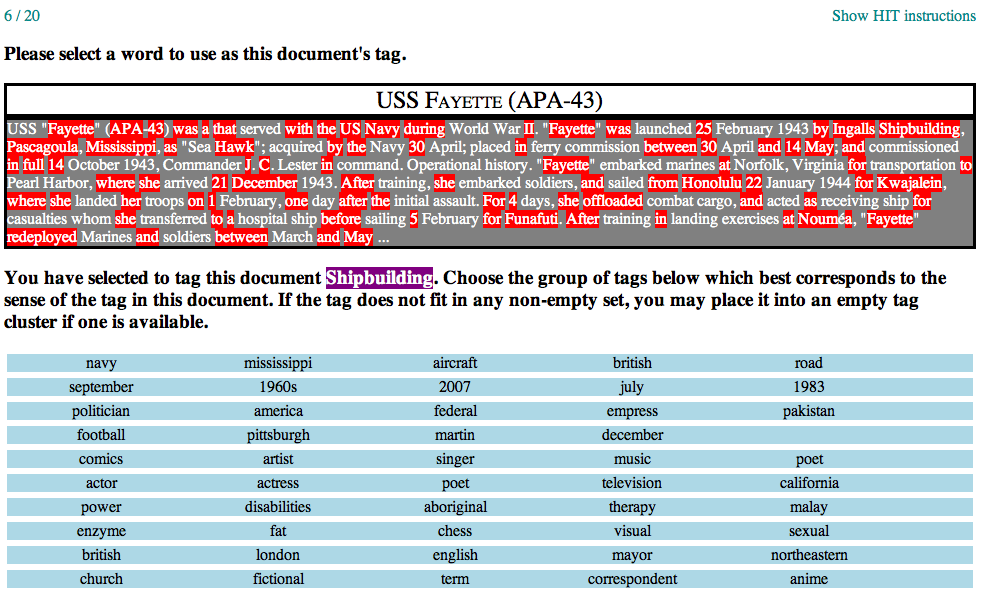
\includegraphics[width=0.90\textwidth]{figures/screenshots.png}
\caption{Screenshots of our task.  In the center, the document along
  with its title is shown.  Words which cannot be selected, e.g.,
  distractors and words previously selected, are shown in red.  Once a
  word is selected, the user is asked to find a topic in which to
  place the word.  The user selects a topic by clicking on an entry in
  a menu of topics, where each topic is expressed by the five words
  which occur most frequently in that topic.}
\label{fig:screenshot}
\end{figure*}

In this task the user is presented with a document along with its
title; the document is randomly selected from a pool of available
documents.  The user is asked to select a word from the document which
is discriminative, i.e, a word which would help someone looking for
the document find it.  Once the word is selected, the user is then
asked to assign the word to the topic which best suits the sense of
the word used in the document.  Users are specifically instructed to
focus on the meanings of words, not their syntactic usage or
orthography.  

The user assigns a word to a topic by selecting an entry out of a menu
of topics.  Each topic is represented by the five words occuring most
frequently in that topic.  The order of the topics presented the user
is determined by the number of words in that document already assigned
to each topic.

Once an instance of a word in a document has been assigned, it cannot
be reassigned and will be marked in red when subsequent users
encounter this document.  In practice, we also prohibit users from
selecting infrequently occurring words and stop words.  


When the set of words minus the intruder makes sense together, then
the subject should easily identify the intruder.  For example, most
people readily identify \word{apple} as the intruding word in the set
\wordset{dog, cat, horse, apple, pig, cow} because the remaining
words, \wordset{dog, cat, horse, pig, cow} make sense together ---
they are all animals.  For the set \wordset{car, teacher, platypus,
  agile, blue, Zaire}, which lacks such coherence, identifying
the intruder is difficult.  People will typically choose an
intruder at random, implying a topic with poor coherence.

